%\begin{frame}
%    \frametitle{\insertsection}
%    \framesubtitle{\insertsubsection}
%
%    \begin{itemize}
%        \item<1-> Strategien zur Resilienzsteigerung in verteilten Systemen
%        \item<2-> Fehlertoleranz und Ausfallsicherheit
%        \item<3-> Praktische Implementierungen wie Circuit Breaker, Retry-Muster
%        \item<4-> Ziel: Absicherung moderner Anwendungen gegen Störungen
%    \end{itemize}
%\end{frame}

\section{Resilienz und Fehlertoleranz}

\subsection{Initiales Beispiel 1.}

\begin{frame}
    \frametitle{\insertsection}
    \framesubtitle{\insertsubsection}
    % SVG beispiel-easy2.svg

\end{frame}

\subsection{Begriffsklärung}

\begin{frame}
    \frametitle{\insertsection}
    \framesubtitle{\insertsubsection}

    \begin{block}{Begriffe}
        \begin{itemize}
            \item \textbf{Resilienz}
                \begin{itemize}
                     \item Funktionsfähigkeit trotz Störungen, Angriffen oder Ausfällen sowie schnelle Erholung\\
                \end{itemize}
            \item \textbf{Fehlertoleranz}
                \begin{itemize}
                    \item Korrektes Funktionieren trotz Fehlern oder Störungen
                \end{itemize}
        \end{itemize}
    \end{block}
\end{frame}


\subsection{Begriffsklärung - Zusammenhang}

\begin{frame}
    \frametitle{\insertsection}
    \framesubtitle{\insertsubsection}

    \begin{block}{Zusammenhang}
        \begin{itemize}
            \item \textbf{Resilienz} = übergeordnetes Konzept, umfasst Fehlertoleranz sowie Aspekte wie Wiederherstellung, Anpassungsfähigkeit und präventive Maßnahmen\\
            \item \textbf{Fehlertoleranz} = Fokus auf unmittelbarer Bewältigung von Fehlern während des Systembetriebs
        \end{itemize}
    \end{block}
\end{frame}

\subsection{Begriffsklärung - Ursprung}

\begin{frame}
    \frametitle{\insertsection}
    \framesubtitle{\insertsubsection}

    %\begin{block}{Ursprung}
        \begin{itemize}
            \item beide Begriffe haben ihren Ursprung nicht in der Informatik
            \item \textbf{Resilienz} aus dem Lateinischen \textit{resilire}, entspricht \glqq zurückspringen\grqq oder  \glqq abprallen\grqq
            \item \textbf{Fehlertoleranz} aus den Ingenieurwissenschaften
        \end{itemize}
    %\end{block}
\end{frame}
%...

\subsection{Motivation}

\begin{frame}
    \frametitle{\insertsection}
    \framesubtitle{\insertsubsection}

    \begin{block}{Motivation}
        \begin{itemize}
            \item Störungen im laufenden Betrieb sollen verhindert werden
            \item Zugunsten der Sicherheit, Kundenzufriedenheit etc.
            %\item Disruption soll vermieden werden
            %\item Reduktion betrieblicher Kosten und Steigerung der Nutzerzufriedenheit
            %\item Anforderungen an Verfügbarkeit in regulierten Branchen
        \end{itemize}
    \end{block}
\end{frame}

%\begin{frame}
%    \frametitle{\insertsection}
%    \framesubtitle{\insertsubsection}
%
%    \begin{itemize}
%        \item Verbreitung von Microservices und Cloud-Technologien
%        \item Herausforderungen durch Kommunikationsausfälle und Spitzenlasten
%        \item Bedarf an innovativen Resilienzmustern
%    \end{itemize}
%\end{frame}

\subsection{Initiales Beispiel 2.}

\begin{frame}
    \frametitle{\insertsection}
    \framesubtitle{\insertsubsection}

    \begin{itemize}
        \item wie können wir Resilienz und Fehlertoleranz am Beispiel weiterführen?
        \item Zunächst natürlich grob, weil die Strategien und Pattern ja noch kommen.
    \end{itemize}
\end{frame}


\section{Strategien}
\subsection{\textbf{Resilienzstrategien}}
\begin{frame}
    \frametitle{\insertsection}
    \framesubtitle{\insertsubsection}

    \begin{itemize}
        \item Redundanz
        \item Partitionierung
        \item Skalierung
    \end{itemize}
\end{frame}

\subsection{Resilienzstrategien: Redundanz}
\begin{frame}
    \frametitle{\insertsection}
    \framesubtitle{\insertsubsection}

    \begin{block}{Definition Redundanz}
        Vervielfältigung kritischer Komponenten oder Funktionen zur Erhöhung der Zuverlässigkeit und Verfügbarkeit.\\
        \begin{itemize}
            \item Unterschiede in Arten der Redundanz und Ebenen der Redundanz.
        \end{itemize}
    \end{block}
\end{frame}


\subsection{Resilienzstrategien: Arten der Redundanz}
\begin{frame}
    \frametitle{\insertsection}
    \framesubtitle{\insertsubsection}
    % \begin{block}{Arten der Redundanz}
        \begin{itemize}
            \item Aktive Redundanz
                \begin{itemize}
                    \item Mehrere Komponenten arbeiten parallel
                    \item Nahtloser Übergang bei Ausfall einer Komponente
                \end{itemize}
            \item Passive Redundanz
                \begin{itemize}
                    \item Redundante Komponenten im Standby.
                    \item Aktivierung bei Ausfall der primären Komponente (mit Umschaltzeit)
                \end{itemize}
        \end{itemize}
   % \end{block}

 %Bild z.B. https://upload.wikimedia.org/wikipedia/commons/8/84/Apollo_15_descends_to_splashdown.jpg

\end{frame}


\subsection{Resilienzstrategien: Ebenen der Redundanz}
\begin{frame}
    \frametitle{\insertsection}
    \framesubtitle{\insertsubsection}

    %\begin{block}{Ebenen der Redundanz}
        \begin{itemize}
            \item Software-Redundanz
            \begin{itemize}
                \item Mehrere Softwarekomponenten erfüllen dieselbe Funktion
            \end{itemize}
            \item Hardware-Redundanz
            \begin{itemize}
                \item Doppelte physische Komponenten (z. B. Netzteile, RAID-Systeme)
            \end{itemize}
            \item Daten-Redundanz
            \begin{itemize}
                \item Mehrfach gespeicherte Daten (z. B. Replikation, Backups)
            \end{itemize}
            \item Netzwerk-Redundanz
            \begin{itemize}
                \item Alternative Übertragungswege (z. B. redundante Router, Glasfaserverbindungen)
            \end{itemize}
            \item Geografische Redundanz
            \begin{itemize}
                \item Verteilung auf mehrere Standorte zur Minimierung großflächiger Ausfälle
            \end{itemize}
        \end{itemize}
   % \end{block}
\end{frame}

\subsection{Resilienzstrategien: Partionierung}
\begin{frame}
    \frametitle{\insertsection}
    \framesubtitle{\insertsubsection}

    \begin{block}{Definition Partionierung}
        Physische Unterteilung von Daten in kleinere, logisch zusammenhängende Einheiten für Skalierbarkeit, Leistung und Flexibilität.
    \end{block}
\end{frame}


\subsection{Resilienzstrategien: Arten der Partionierung}
\begin{frame}
    \frametitle{\insertsection}
    \framesubtitle{\insertsubsection}
  %  \begin{block}{Arten der Partionierung}
        \begin{itemize}
            \item Horizontale Partitionierung: Aufteilung von Datensätzen basierend auf einem Partitionsschlüssel
            \item Vertikale Partitionierung: Gruppierung von Spalten einer Tabelle
            \item Funktionale Partitionierung: Organisation nach Funktion oder Zweck der Daten
            \item RANGE-Partitionierung: Unterteilung nach Wertebereichen (z. B. Zeit, Zahlen)
            \item HASH-Partitionierung: Verteilung durch Hash-Funktion für gleichmäßige Last
            \item Round-Robin Partitioning: Gleichmäßige, zyklische Datenverteilung
        \end{itemize}
  %  \end{block}
\end{frame}

% Bild Partitionierung nicht gut aber z.B. https://www.flip-design.de/wp-content/uploads/2011/04/SQLServerPartitionierung.png


\subsection{Resilienzstrategien: Skalierung}
\begin{frame}
    \frametitle{\insertsection}
    \framesubtitle{\insertsubsection}

    \begin{block}{Definition Skalierung}
Flexible Anpassung von Ressourcen an veränderte Anforderungen.
    \end{block}
\end{frame}

\subsection{Resilienzstrategien: Arten der Skalierung}
\begin{frame}
    \frametitle{\insertsection}
    \framesubtitle{\insertsubsection}

   %\begin{block}{Arten der Skalierung}
        \begin{itemize}
            \item Vertikale Skalierung (Scale Up)
            \begin{itemize}
                \item Aufrüstung von Hardware (z. B. CPU, RAM) eines Systems
                \item Begrenzung auf eine zentrale Einheit
            \end{itemize}
            \item Horizontale Skalierung (Scale Out):
            \begin{itemize}
                \item Hinzufügen von Servern oder Instanzen
                \item Verteilte Last auf mehrere Einheiten
            \end{itemize}
            \item Automatische Skalierung:
            \begin{itemize}
                \item Dynamische Anpassung der Ressourcen
                \item Häufig in Cloud-Umgebungen für optimierte Ressourcennutzung
            \end{itemize}
        \end{itemize}
  %\end{block}
\end{frame}

% Bild Skalierung z.B. https://www.shutterstock.com/search/scalability-logo


\subsection{\textbf{Pattern für Fehlertoleranzstrategien}}

\begin{frame}
    \frametitle{\insertsection}
    \framesubtitle{\insertsubsection}

    \begin{itemize}
        \item Fehlerbehandlung und -isolierung mittels Retry-Pattern
        \item Nutzung von Fallback-Mechanismen
        \item Vermeidung kaskadierender Fehler mittels Circuit-Breaker
    \end{itemize}
\end{frame}


\section{Pattern und Konzepte}
\subsection{\textbf{Circuit-Breaker}}

\begin{frame}
    \frametitle{\insertsection}
    \framesubtitle{\insertsubsection}
    \begin{block}{Definition - Was ist ein Circuit-Breaker?}
        Entwurfsmuster zur Isolation fehlerhafter Dienste in verteilten Systemen, um Überlastung zu verhindern
        und Stabilität zu gewährleisten.
        % TODO das ist gerade noch ziemlich redundant (Definition, Aufgaben, Vorteile) geht vielleicht differenzierter
    \end{block}
    \begin{block}{Aufgaben}
        \begin{itemize}
            \item Isoliert fehlerhafte Dienste
            \item Unterbricht Anfragen bei wiederholtem Fehler
            \item Verhindert kaskadierende Ausfälle
        \end{itemize}
    \end{block}
\end{frame}

\subsection{Circuit-Breaker: Zustandsdiagramm}
\begin{frame}
    \frametitle{\insertsection}
    \framesubtitle{\insertsubsection}

    \begin{figure}
        \pgfdeclarelayer{background}
        \pgfdeclarelayer{foreground}
        \pgfsetlayers{background,main,foreground}
    % Define a few styles and constants
        \tikzstyle{state} = [draw, rounded corners,
        text centered, minimum height=3em, minimum width=4em]
        \centering
        \centering
        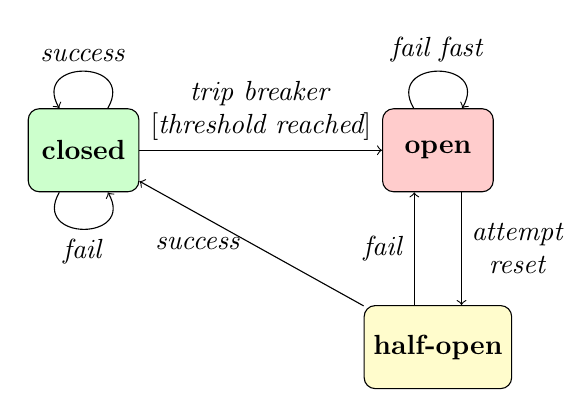
\begin{tikzpicture}[
    %scale=0.6, every node/.style={scale=0.6}
        ]
            \node (closed) [state, fill=green!20] {\textbf{closed}};
            \node (open) [state, fill=red!20, right of=closed, node distance =4.5cm] {\textbf{open}};
            \node (halfopen) [state, fill=yellow!20, below of=open, node distance =2.5cm] {\textbf{half-open}};
            \draw [->] (closed) -- (open) node[above,midway,align=center] {\textit{trip breaker}\\\textit{$[$threshold
            reached$]$}};
            \draw [->] (halfopen) -- (closed) node[left,midway] {\textit{success}};
            \draw [transform canvas={xshift=-0.3cm},->] (halfopen) -- (open) node[left,midway] {\textit{fail}};
            \draw [transform canvas={xshift=0.3cm},->] (open) -- (halfopen) node[right,midway,align=center]
                {\textit{attempt}\\\textit{reset}};
            \path[]	(open)   edge[loop, in=60,out=120, looseness=3,->] node[above]  {\textit{fail fast}} (open);
            \path[]	(closed)   edge[loop, in=60,out=120, looseness=3,<-] node[above]  {\textit{success}} (closed);
            \path[]	(closed)   edge[loop, in=240,out=300, looseness=3,<-] node[below]  {\textit{fail}} (closed);
        \end{tikzpicture}
        \caption{Circuit Breaker Zustandsdiagramm} % TODO Quelle
        \label{cb-fsm}
    \end{figure}
\end{frame}


\subsection{Circuit-Breaker: Implementierungsansätze}
\begin{frame}
    \frametitle{\insertsection}
    \framesubtitle{\insertsubsection}

    \begin{itemize}
        \item Clientseitig
        \begin{itemize}
            \item Abfangen externer Anfragen vor der Weiterleitung
        \end{itemize}
        \item Dienstseitig
        \begin{itemize}
            \item Schutz des Dienstes vor Überlastung durch viele fehlerhafte Anfragen
        \end{itemize}
        \item Proxy-basiert
        \begin{itemize}
            \item Circuit-Breaker zwischen Clients und Diensten in Proxys platziert
        \end{itemize}
    \end{itemize}
\end{frame}


\subsection{Circuit-Breaker: Vorteile}
\begin{frame}
    \frametitle{\insertsection}
    \framesubtitle{\insertsubsection}

    \begin{itemize}
        \item Verhindert kaskadierende Ausfälle in verteilten Systemen
        \item Verbesserte Systemstabilität durch Isolierung fehlerhafter Dienste
        \item Bessere Benutzererfahrung durch Fallback-Mechanismen
        \item Unterstützt Resilienz und Wiederherstellung in kritischen Systemen
    \end{itemize}
\end{frame}

\subsection{Circuit-Breaker: Nachteile}
\begin{frame}
    \frametitle{\insertsection}
    \framesubtitle{\insertsubsection}

    \begin{itemize}
        \item Erhöhte Komplexität in der Implementierung und Wartung
        \item Risiko von Fehlkonfiguration (z. B. falsche Schwellenwerte)
        \item Zusätzlicher Overhead durch Überwachung und Statusverwaltung
        \item Fallback-Daten können veraltet oder ungenau sein
    \end{itemize}
\end{frame}

\subsection{Circuit-Breaker: großes Diagramm mit Anpassungen}
\begin{frame}
    \frametitle{\insertsection}
    \framesubtitle{\insertsubsection}

\end{frame}

%\subsection{\textbf{Retry-Muster}}
%\begin{frame}
 %   \frametitle{\insertsection}
  %  \framesubtitle{\insertsubsection}

%   \begin{itemize}
 %       \item Automatisches Wiederholen fehlgeschlagener Operationen
  %      \item Nutzung von Exponential Backoff
   %     \item Verbesserung der Resilienz bei temporären Fehlern
    %\end{itemize}
%\end{frame}

\subsection{\textbf{Retry-Muster}}
\begin{frame}
    \frametitle{\insertsection}
    \framesubtitle{\insertsubsection}
    \begin{block}{Definition - Was ist ein Retry-Muster?}
        Architekturmuster zur automatischen Wiederholung fehlgeschlagener Operationen, insbesondere bei vorübergehenden Fehlern.
    \end{block}
    \begin{block}{Funktionen}
        \begin{itemize}
            \item Handhabt vorübergehende Fehler durch wiederholte Versuche
            \item Nutzt dazu exponentielle Backoff-Strategien (= Verlängerung der Wartezeit zwischen Wiederholungen)
        \end{itemize}
    \end{block}
\end{frame}

\subsection{Retry-Muster: Sequenzdiagramm}
\begin{frame}
    \frametitle{\insertsection}
    \framesubtitle{\insertsubsection}

    \begin{figure}[h]
        \centering
        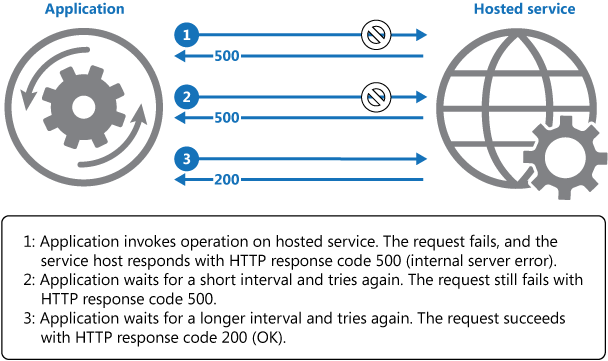
\includegraphics[height=0.5\textheight]{../images/retry-pattern}
        \caption{Sequenzdiagramm des Retry Patterns}
    \end{figure}
\end{frame}

\subsection{Retry-Muster: Vorteile}
\begin{frame}
    \frametitle{\insertsection}
    \framesubtitle{\insertsubsection}

    \begin{itemize}
    \item Reduziert die Wahrscheinlichkeit eines vollständigen Anwendungsabsturzes bei vorübergehenden Fehlern.
    \item Verbessert die Zuverlässigkeit, indem kurzfristige Probleme (z. B. Netzwerkprobleme) automatisch überwunden werden.
    \item Ermöglicht ein einheitliches Fehlerbehandlungsmodell in einer Anwendung.
\end{itemize}
\end{frame}

\subsection{Retry-Muster: Nachteile}
\begin{frame}
    \frametitle{\insertsection}
    \framesubtitle{\insertsubsection}

    \begin{itemize}
        \item Erhöhte Komplexität in der Implementierung und Wartung.
        \item Verzögert die Gesamtverarbeitung, wenn ein Vorgang wiederholt fehlschlägt.
        \item Kann echte, dauerhafte Fehler verschleiern, wenn nur wiederholt wird, ohne die Ursache zu analysieren.
        \item Nicht jeder Fehler ist vorübergehend (z. B. Authentifizierungsfehler), was zu unnötigen Wiederholungen führt.
    \end{itemize}
\end{frame}

\subsection{\textbf{Kombination mit Circuit-Breaker}}

\begin{frame}
    \frametitle{\insertsection}
    \framesubtitle{\insertsubsection}

    \begin{itemize}
        \item Stoppt Wiederholungen bei permanenten Fehlern
        \item Ermöglicht Systemen, sich zu erholen
        \item Optimiert Ressourcennutzung
    \end{itemize}
\end{frame}


\subsection{\textbf{Load Balancing}}
\begin{frame}
    \frametitle{\insertsection}
    \framesubtitle{\insertsubsection}
    \begin{block}{Definition - Was ist Load-Balancing?}
        Verteilung der Last auf mehrere Server zur Verbesserung von Leistung und Ausfallsicherheit
    \end{block}
    \begin{block}{Arten}
        \begin{itemize}
       		\item Network Load Balancer
       		\item Application Load Balancer
        	\item Hardware Load Balancer
         \end{itemize}
    \end{block}
\end{frame}

\subsection{Load Balancing: Service Discovery}
\begin{frame}
	\frametitle{\insertsection}
    \framesubtitle{\insertsubsection}
    \begin{block}{Service Discovery}
	\begin{itemize}
		\item \textbf{Server-side Discovery}
		\begin{itemize}
			\item Ein zentraler Load Balancer
			\item Dienste sind unsichtbar für Client
		\end{itemize}
			\item \textbf{Client-side Discovery}
		\begin{itemize}
			\item Kein zentraler Load Balancer
			\item Client sieht alle Dienstinstanzen
			\item Client betreibt Load Balancing
		\end{itemize}
	\end{itemize}
    \end{block}
\end{frame}

\subsection{Load Balancing: Architekturdiagramm}
\begin{frame}
    \frametitle{\insertsection}
    \framesubtitle{\insertsubsection}
    \begin{columns}[c]
        \begin{column}{0.4\textwidth}
	        \begin{block}{Komponenten}
	            \begin{itemize}
	                \item Load Balancer
	                \item Service Registry
	                \item Dienstinstanzen
	            \end{itemize}
	        \end{block}
        \end{column}
        \begin{column}{0.6\textwidth}
        	\begin{figure}[h]
	            \centering
	            \captionsetup{aboveskip=2pt}
	            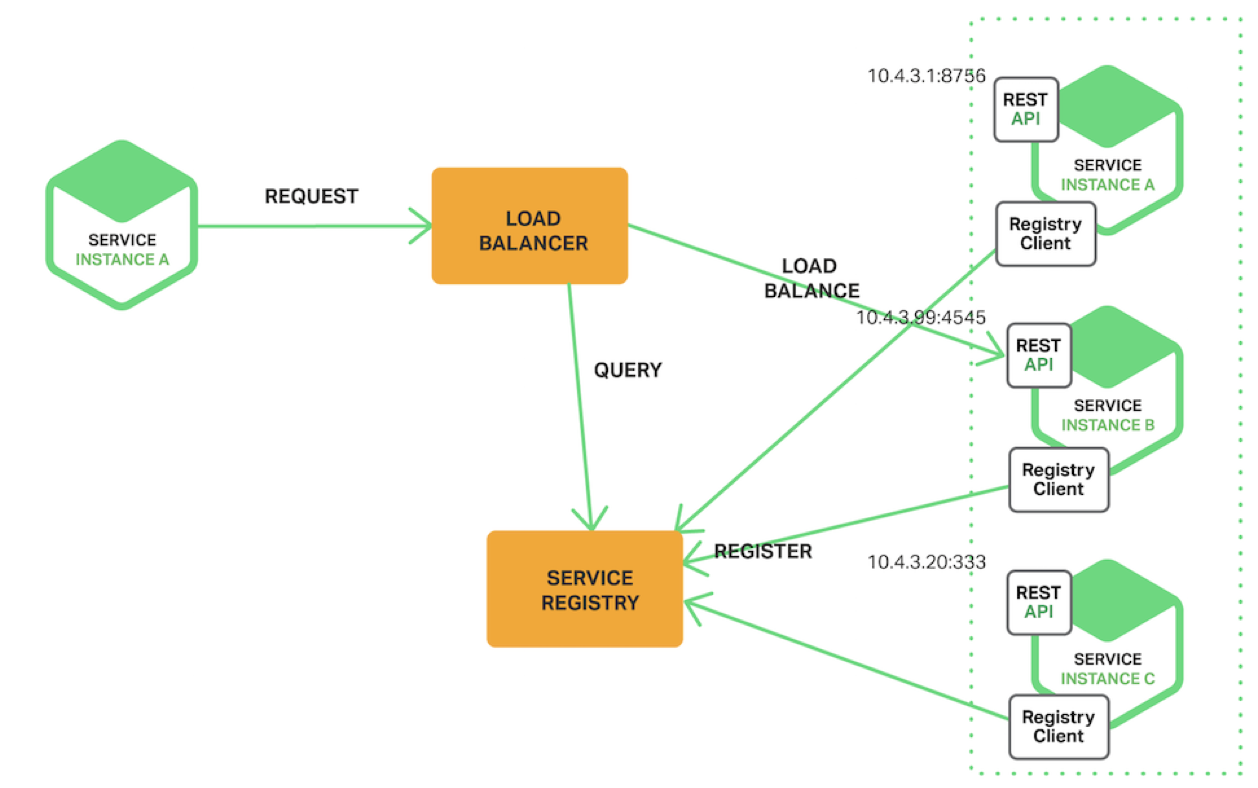
\includegraphics[width=.95\linewidth]{../images/loadbalancer}  
	            \caption{Load Balancer mit Server Side Discovery}      		
        	\end{figure}
        \end{column}
    \end{columns}
\end{frame}

\subsection{Load Balancing: statische Strategien}
\begin{frame}
    \frametitle{\insertsection}
    \framesubtitle{\insertsubsection}
    \begin{block}{Source IP Hash Load Balancing}
        \begin{itemize}
            \item Clients werden praktisch zufällig verteilt
            \item Anfragen eines Clients werden immer auf der selben Serviceinstanz verarbeitet (\textit{Sticky Sessions})
        \end{itemize}
    \end{block}
    \begin{block}{Round Robin}
        \begin{itemize}
            \item Anfragen werden zyklisch auf Instanzen verteilt
        \end{itemize}
    \end{block}
\end{frame}

\subsection{Load Balancing: dynamische Strategien}
\begin{frame}
    \frametitle{\insertsection}
    \framesubtitle{\insertsubsection}
    \begin{block}{Least Connection}
        \begin{itemize}
            \item Anstehende Aufgabe geht an den Dienst mit den momentan wenigsten aktiven Netzwerkverbindungen
            % https://www.researchgate.net/publication/347808307/figure/fig2/AS:1000876902723590@1615639057440/Least-connection-algorithm.png
        \end{itemize}
    \end{block}
    \begin{block}{Resource Based}
        \begin{itemize}
            \item Serviceknoten berichten aktuelle Auslastung (z.B. CPU-Auslastung)
            \item Nächste Aufgabe geht an den Knoten mit niedrigster Auslastung
        \end{itemize}
    \end{block}
\end{frame}

\begin{frame}
    \frametitle{\insertsection}
    \framesubtitle{\insertsubsection}

    \begin{figure}[h]
        \centering
        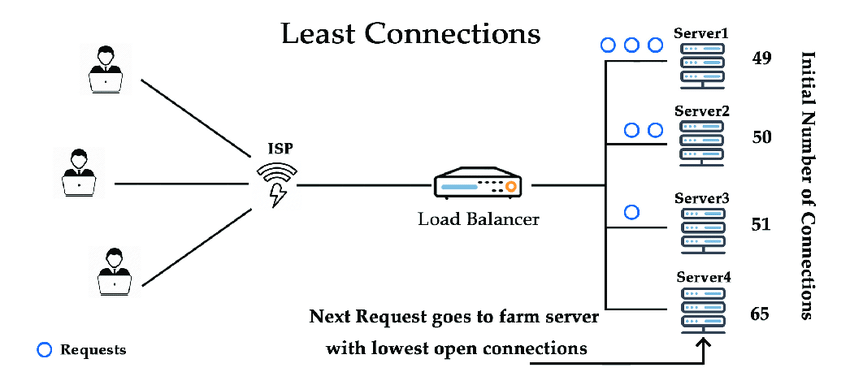
\includegraphics[height=0.55\textheight]{../images/leastconnection}
        \caption{Least Connection-basiertes Load Balancing}
    \end{figure}
\end{frame}

\subsection{Health Checks bei Load Balancing}
\begin{frame}
    \frametitle{\insertsection}
    \framesubtitle{\insertsubsection}

    \begin{itemize}
    	\begin{block}{Konzept}
    		Dienstinstanzen kommunizieren ihren Grad der Funktionsbereitschaft, um dynamische Lastverteilung zu ermöglichen.
    	\end{block}

        \item Dienste haben Endpunkte, um Auslastung oder Fehler abzurufen
        \item Überlastete Dienste erhalten weniger Anfragen
        \item Fehlerhafte Dienste können übergangen werden
    \end{itemize}
\end{frame}

\subsection{Load Balancing: dynamische Skalierung}
\begin{frame}
    \frametitle{\insertsection}
    \framesubtitle{\insertsubsection}
    
    \begin{block}{Problem}
	    \begin{itemize}
	    	\item Die Anzahl der Anfragen ist nicht immer gleich
	   		\begin{itemize}
	   			\item Zur Spitzenbelastung sind mehr Dienstknoten nötig
	   			\item In Ruhezeiten verschwenden unterbelastete Knoten Strom und Geld
	   		\end{itemize}
	    \end{itemize}
    \end{block}
    
    \begin{block}{Die Lösung: dynamische Skalierung}
		\begin{itemize}
			\item Der Load Balancer wird befähigt, Dienstinstanzen zu starten und stoppen
			\item Schwellwerte definieren, wann dies erfolgen soll
		\end{itemize}	
    \end{block}

\end{frame}

\subsection{Load Balancing: Vorteile}
\begin{frame}
    \frametitle{\insertsection}
    \framesubtitle{\insertsubsection}
    
    \begin{itemize}
    	\item Gesteigerter Durchsatz durch parallel laufende Dienste
    	\item Hohe Verfügbarkeit durch Redundanz und nahtlosem Failover
    	\item Kostenreduktion durch dynamische horizontale Skalierung
    \end{itemize}
\end{frame}

\subsection{Load Balancing: Nachteile}
\begin{frame}
    \frametitle{\insertsection}
    \framesubtitle{\insertsubsection}
    
    \begin{itemize}
    	\item Deutlich gesteigerte Komplexität der Infrastruktur
    	\item Zusätzliche Kosten für Load Balancer (Hardware und Lizenz)% hier dann latenz bei zu schwachem LB erwähnen (LB auch nur vertikal skalierbar)
    	\item Dienste sind nicht immer kompatibel
		\begin{itemize}
			\item Healthchecks müssen implementiert werden
			\item Stateful-Dienste sind nur eingeschränkt verwendbar
		\end{itemize}
    	\item Anstelle eines einzelnen Dienstes ist jetzt der Load Balancer ein Single~Point~of~Failure
    \end{itemize}
\end{frame}

\subsection{Round Robin DNS}
\begin{frame}
    \frametitle{\insertsection}
    \framesubtitle{\insertsubsection}
    \begin{block}{Definition - was ist Round Robin DNS?}
    \begin{itemize}
        \item Für eine Domain werden mehrere IP-Adressen hinterlegt
        \item DNS-Server gibt alle Adressen in rotierender Reihenfolge zurück

%        \item Verteilt so Lasten und erhöht Verfügbarkeit

        % https://www.cloudns.net/images/wiki/Round-Robin-DNS.png
    \end{itemize}
    \end{block}
    \begin{block}{Wirkung}
    	\begin{itemize}
    		\item Externes, statisches Load Balancing
    		\item Verfügbarkeit auch bei Totalausfall eines Servers
    	\end{itemize}
    \end{block}
\end{frame}


\begin{frame}
    \frametitle{\insertsection}
    \framesubtitle{\insertsubsection}

    \begin{figure}[h]
        \centering
        \captionsetup{aboveskip=0pt}
        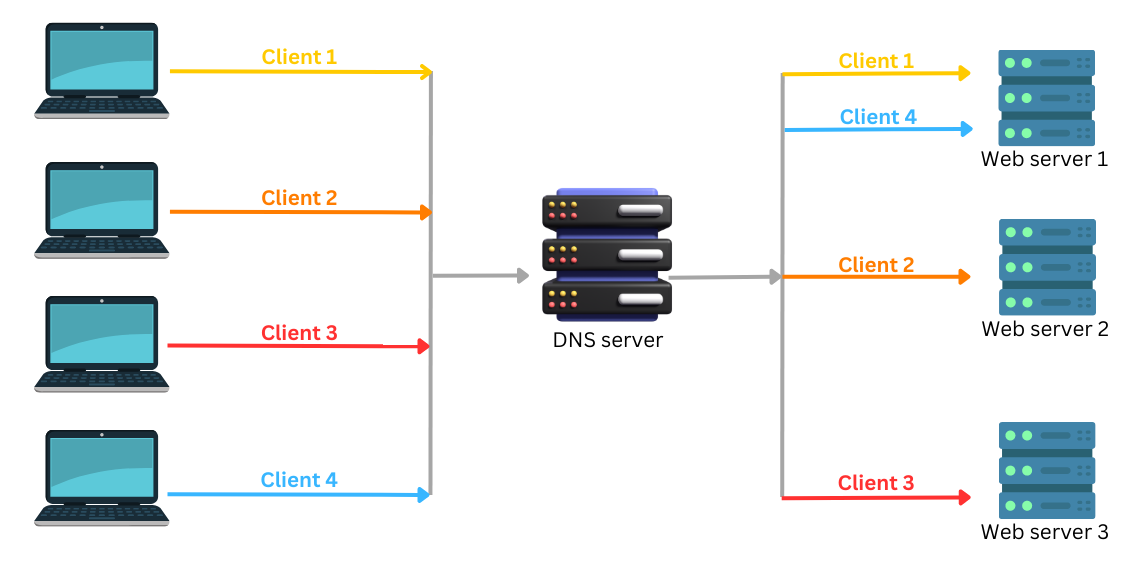
\includegraphics[width=.7\textwidth]{../images/roundrobindns}
        \caption{Round Robin DNS}
    \end{figure}
\end{frame}

\subsection{Round Robin DNS: Vorteile}
\begin{frame}
    \frametitle{\insertsection}
    \framesubtitle{\insertsubsection}
    
    \begin{itemize}
    	\item Einfach zu implementieren
    	\item Sticky Sessions by default
    	\item Fallback auf eine andere IP-Adresse schützt auch bei einem Serverausfall
    \end{itemize}
\end{frame}

\subsection{Round Robin DNS: Nachteile}
\begin{frame}
    \frametitle{\insertsection}
    \framesubtitle{\insertsubsection}
    
    \begin{block}{Balancing}
	    \begin{itemize}
	    	\item Nur statische Lastverteilung ist möglich
	    	\item Die Reihenfolge der IPs wird vom DNS ein Mal bestimmt, aber danach gecached
	    	\begin{itemize}
	    		\item Verteilung kann zufällig ungleich werden, da Balancing nur unregelmäßig erfolgt
	    		\item Neue Server erst nach gewisser Zeit gleich stark ausgelastet
	    	\end{itemize}
	    \end{itemize}
    \end{block}
    
    \begin{block}{Failover-Verhalten}
	    \begin{itemize}
	    	\item Vom Client kontrolliert, nicht vom Server oder DNS
	    	\begin{itemize}
	    		\item Lange Wartezeiten bis zum Failover sind möglich
	    	\end{itemize}
	    \end{itemize}
    \end{block}

\end{frame}

\section{Fazit}
\subsection{Was wurde gemacht?}

\begin{frame}
    \frametitle{\insertsection}
    \framesubtitle{\insertsubsection}

    \begin{itemize}
        \item Analyse und Implementierung von Resilienzstrategien
        \item Fallstudien und Praxisbeispiele
        \item Implementierungen in Python
    \end{itemize}
\end{frame}

\subsection{Fallstudie: Netflix}
\begin{frame}
    \frametitle{\insertsection}
    \framesubtitle{\insertsubsection}

    \begin{itemize}
        \item Nutzung von Hystrix für Circuit-Breaker
        \item Dynamisches Load Balancing
        \item Skalierung und Fehlertoleranz
    \end{itemize}
\end{frame}

%\section{Ausblick}
%
%\begin{frame}
%    \frametitle{\insertsection}
%    \framesubtitle{\insertsubsection}
%
%    \begin{itemize}
%        \item Circuit Breaker und Retry-Muster als effektive Mechanismen
%        \item Kombination verschiedener Strategien verbessert Resilienz
%        \item Bedeutung von agilen Methoden zur kontinuierlichen Verbesserung
%    \end{itemize}
%\end{frame}

\section{Diskussion}

\begin{frame}
    \frametitle{\insertsection}
    \framesubtitle{\insertsubsection}

    \begin{itemize}
        \item Erweiterung der Strategien auf andere Szenarien
        \item Entwicklung neuer Muster zur Resilienzsteigerung
        \item Untersuchung ökonomischer Auswirkungen
    \end{itemize}
\end{frame}

\section{Quellen}
\begin{frame}[allowframebreaks]{\insertsection} % Allow frame breaks if many references
\bibliography{../literatur}
\end{frame}

\section{Cheatsheet zum Lernen}

\begin{frame}
\frametitle{\insertsection}
\framesubtitle{\insertsubsection}

\begin{itemize}
    \item TODO, damit hätten wir etwas, was noch keine Gruppe hat.
    \item die wichtigsten Definitionen usw hier in kleinerer Schrift (tiny)
\end{itemize}
\end{frame}

\begin{frame}[shrink=10]{Cheatsheet: Wichtige Definitionen und Konzepte}
    \scriptsize
    \justifying

    \begin{columns}[t]
        \column{0.3\textwidth}
        \textbf{1. Grundbegriffe}\\
        \textbf{Resilienz} = Übergeordnetes Konzept, Fehlertoleranz + Aspekte wie
        Wiederherstellung, Anpassungsfähigkeit und präventive Maßnahmen\\
        \textbf{Fehlertoleranz} = Fokus auf unmittelbarer Bewältigung von Fehlern während des
        Systembetriebs\\
        \textbf{Ziel}: Störungen im laufenden Betrieb vermeiden

        \column{0.3\textwidth}
        \textbf{2. Resilienzstrategien}\\
            \textbf{Redundanz}: Vervielfältigung kritischer Komponenten oder Funktionen zur Erhöhung der
            Zuverlässigkeit und Verfügbarkeit.\\
        -> aktive vs. passive Redundanz; Redundanzebenen!\\
            \textbf{Partionierung}: Physische Unterteilung von Daten in kleinere, logisch zusammenhängende Einheiten
            für Skalierbarkeit, Leistung und Flexibilität.\\
            \textbf{Skalierung}: Flexible Anpassung von Ressourcen an veränderte Anforderungen.\\
        -> vertikal vs. horizontal vs. automatisch!


        \column{0.3\textwidth}
        \textbf{3. Fehlertoleranzstrategien + Pattern}
            \textbf{Retry-Muster}: Wiederholt fehlgeschlagene Operationen, oft mit Backoff-Strategien.\\
            \textbf{Circuit-Breaker}: Isoliert fehlerhafte Dienste, unterbricht Anfragen bei wiederholtem Fehler,
            verhindert kaskadierende Ausfälle.\\
        -> clientseitig vs. dienstseitig vs. proxy-basiert!\\
            \textbf{Load-Balancing}: Verteilung der Last auf mehrere Server zur Verbesserung von Leistung und
            Ausfallsicherheit.\\
            \textbf{Load-Balancing-Strategien}:
            \begin{itemize}
                \item Round Robin DNS: rotierende Rückgabe von IP-Adressen
                \item Least Connection: Aufgabe an Dienst mit den wenigsten aktiven Netzwerkverbindungen
            %    \item Recource Based: Aufgabe an Knoten mit geringster Auslastung
            \end{itemize}
    \end{columns}
\end{frame}
